\documentclass[25pt, a0paper, portrait]{tikzposter}
\tikzposterlatexaffectionproofoff %% remove the mark on the bottom right

\usepackage{hyperref}
\usepackage{booktabs}
\usepackage{adjustbox}
\usepackage{multicol}
\usepackage{listings}
\usepackage{stmaryrd, amssymb, amsmath}
\usepackage{xspace}

\usepackage{paralist}

\usetikzlibrary{arrows.meta}
\tikzset{>={Latex[width=6mm,length=10mm]}}

\usepackage{color,soul} %% highlighting


\definecolor{Black}{RGB}{0,0,0}

\RequirePackage[T1]{fontenc}
\RequirePackage{fontspec}
\fontspec[AutoFakeBold=3.5]{IMFellEnglish-Regular.ttf}

%% Font of the text, might use a different one for the title
%% that matches better the New York Times front page.
\setmainfont{IMFellEnglish}[
  Path=./,
  UprightFont = *-Regular.ttf,
  ItalicFont = *-Italic.ttf,
  BoldFont= *-Regular.ttf,
  BoldFeatures={FakeBold=3.5},
  SmallCapsFont=Chomsky.otf,
]

\newcommand*\hlbis[1]{%
    \tikz[baseline,%
      decoration={random steps,amplitude=4pt,segment length=25pt},%
      outer sep=-0.1em, inner sep = 0pt%
    ]%
   \node[decorate,rectangle,fill=yellow,anchor=text]{#1\xspace};%
}%

%% Custom background and frame, we only need it to be white
\definebackgroundstyle{samplebackgroundstyle}{
  \draw[inner sep=0pt, line width=0pt, color=white, fill=white]
  (bottomleft) rectangle (topright);
}

%% Custom title, nothing really, just remove the ugly frame
\definetitlestyle{sampletitlestyle}{
  width=500mm, roundedcorners=20, linewidth=2pt, innersep=5pt,
  titletotopverticalspace=15mm, titletoblockverticalspace=30mm
}{}

%% Custom block style, we want a title and that's it.
\defineblockstyle{sampleblockstyle}{
    titlewidthscale=1, bodywidthscale=1, titleleft,
    titleoffsetx=0pt, titleoffsety=0pt, bodyoffsetx=0pt, bodyoffsety=0pt,
    bodyverticalshift=0pt, roundedcorners=0,
    titleinnersep=0.5cm, bodyinnersep=0.5cm
}{ %% nothing really
}

%% Colors
\definecolorstyle{samplecolorstyle} {
  \definecolor{colorOne}{named}{yellow}
  \definecolor{colorTwo}{named}{black}
  \definecolor{colorThree}{named}{cyan}
} {
  \colorlet{backgroundcolor}{colorOne}
  \colorlet{framecolor}{black}
  \colorlet{blocktitlefgcolor}{black}
  \colorlet{blocktitlebgcolor}{white}
}

\definelayouttheme{sample}{
  \usecolorstyle{samplecolorstyle}
  \usetitlestyle{sampletitlestyle}
  \usebackgroundstyle{samplebackgroundstyle}
  \useblockstyle{sampleblockstyle}
  \useinnerblockstyle{sampleblockstyle}
}

\usetheme{sample}


\makeatletter
\renewcommand\Huge{\@setfontsize\Huge{220}{220}} %% big title
\renewcommand\huge{\@setfontsize\Huge{120}{120}}
\renewcommand\LARGE{\@setfontsize\Huge{70}{70}}
\renewcommand\Large{\@setfontsize\Huge{60}{60}}
\renewcommand\large{\@setfontsize\Huge{50}{50}}
\renewcommand\normalsize{\@setfontsize\Huge{40}{40}} %% between 24-36
\renewcommand\small{\@setfontsize\Huge{33}{33}}
\renewcommand\footnotesize{\@setfontsize\Huge{15}{15}}
\renewcommand\scriptsize{\@setfontsize\Huge{12}{12}}
\renewcommand\tiny{\@setfontsize\Huge{10}{10}} 
\makeatother

\newcommand{\TOPBLOCK}{0.17}

\newcommand*{\myfont}{\fontfamily{scfamily}\selectfont}
\newcommand*{\oldfont}{\fontfamily{rmfamily}\selectfont}

\settitle{
  \vspace{-1em}
  \centering
  \begin{tabular}{p{\TOPBLOCK\columnwidth}p{0.62\columnwidth}p{\TOPBLOCK\columnwidth}}
    \adjustbox{max width=\TOPBLOCK\columnwidth}{\fbox{\parbox{\dimexpr\linewidth-2\fboxsep-2\fboxrule}
        {``\@author ~ from \textit{\@institute}''}}} &
    \centering\Huge\scshape\@title &
    \adjustbox{max width=\TOPBLOCK\columnwidth}{{\parbox{\dimexpr\linewidth-2\fboxsep-2\fboxrule}{
          \begin{center}
            \textbf{ISWC edition}
          \end{center}
          
          The 22$^{nd}$ International Semantic Web Conference: The
          premier international forum for the Semantic Web and Linked
          Data Community.}}} \vspace{0.25em}\\ \midrule
    
    & \centering\uppercase{Athens, Greece, 6-10 November 2023} & \hfill\$0.00\\ \bottomrule
  \end{tabular}
}

\newcommand{\HRULE}{\centerline{\rule{0.4\linewidth}{0.1cm}}}
\newcommand{\VRULE}{\draw[line width=0.2cm] (blocktitle.north east) -- (blockbody.south east);}
\newcommand{\VRULELEFT}{\draw[line width=0.2cm]
  ([xshift=-1cm]blocktitle.north west) -- ([xshift=-1cm]blockbody.south west);}




\title{Raw-Jena}

\author{Julien Aimonier-Davat and Minh-Hoang Dang and Pascal Molli and Brice Nédelec and Hala Skaf-Molli}
\date{November 6--10}
\institute{Nantes Université, CNRS, LS2N}

\setlength{\columnsep}{1.5cm}

\begin{document}
\maketitle[width=\columnwidth]

\begin{columns}
  \column{0.74}
  \block{\huge Approximate Query Processing for SPARQL Endpoints}{
    \begin{multicols}{2}
      \begin{center}
        \HRULE
        \textit{Integrate sampling as SQL did with the TABLESAMPLE clause.}
        \HRULE
      \end{center}
      
      \hlbis{Sampling-based approximate query pro-}
      \hlbis{cessing (S-AQP)} [1]
      has many important use cases for RDF such as computing
      \begin{itemize}
      \item large-scale statistics,
      \item knowledge graph embeddings,
      \item join orders,
      \item approximate aggregations,
      \item summaries,
      \item exploratory queries.
      \end{itemize}
      \ \\
      By confining query execution to samples of large datasets,
      S-AQP drastically
      \begin{itemize}
      \item \hlbis{reduces} execution time, 
      \item delivering \hlbis{approximate results}
      \item with \hlbis{error} estimates.
      \end{itemize}
    \end{multicols}%
  }
  \VRULE
  %
  \column{0.26}
  \block{Ad-hoc sampling}{
    \begin{center}
      \HRULE
      \textit{exists in a few engines~[A,B] and it is not great!}
      \HRULE
      
      \uppercase{May \hlbis{time out} on public SPARQL endpoints\ldots}
      \HRULE
    \end{center}
    
    \texttt{SELECT * \{?s ?p ?o\} OFFSET r LIMIT 1}, where $r$ is a
    random number between 0 and the dataset size (0 $< r <$ 12B).\\

%    Sampling and random exist in a few engines~[A, B].
    
    %% Well-known engines such as
    %% Stardog\footnote{\url{https://docs.stardog.com/query-stardog/sampling-service\#sampling-service}},
    %% or
    %% Virtuoso\footnote{https://docs.openlinksw.com/virtuoso/rndsalltr/},
    %% propose an ad-hoc sampling API, but with no guarantee on complexity.\\
  }
  % \VRULELEFT
\end{columns}



\block{Random walks for cardinality estimates and confidence with Wander~Join~[2]}{
  \fbox{
    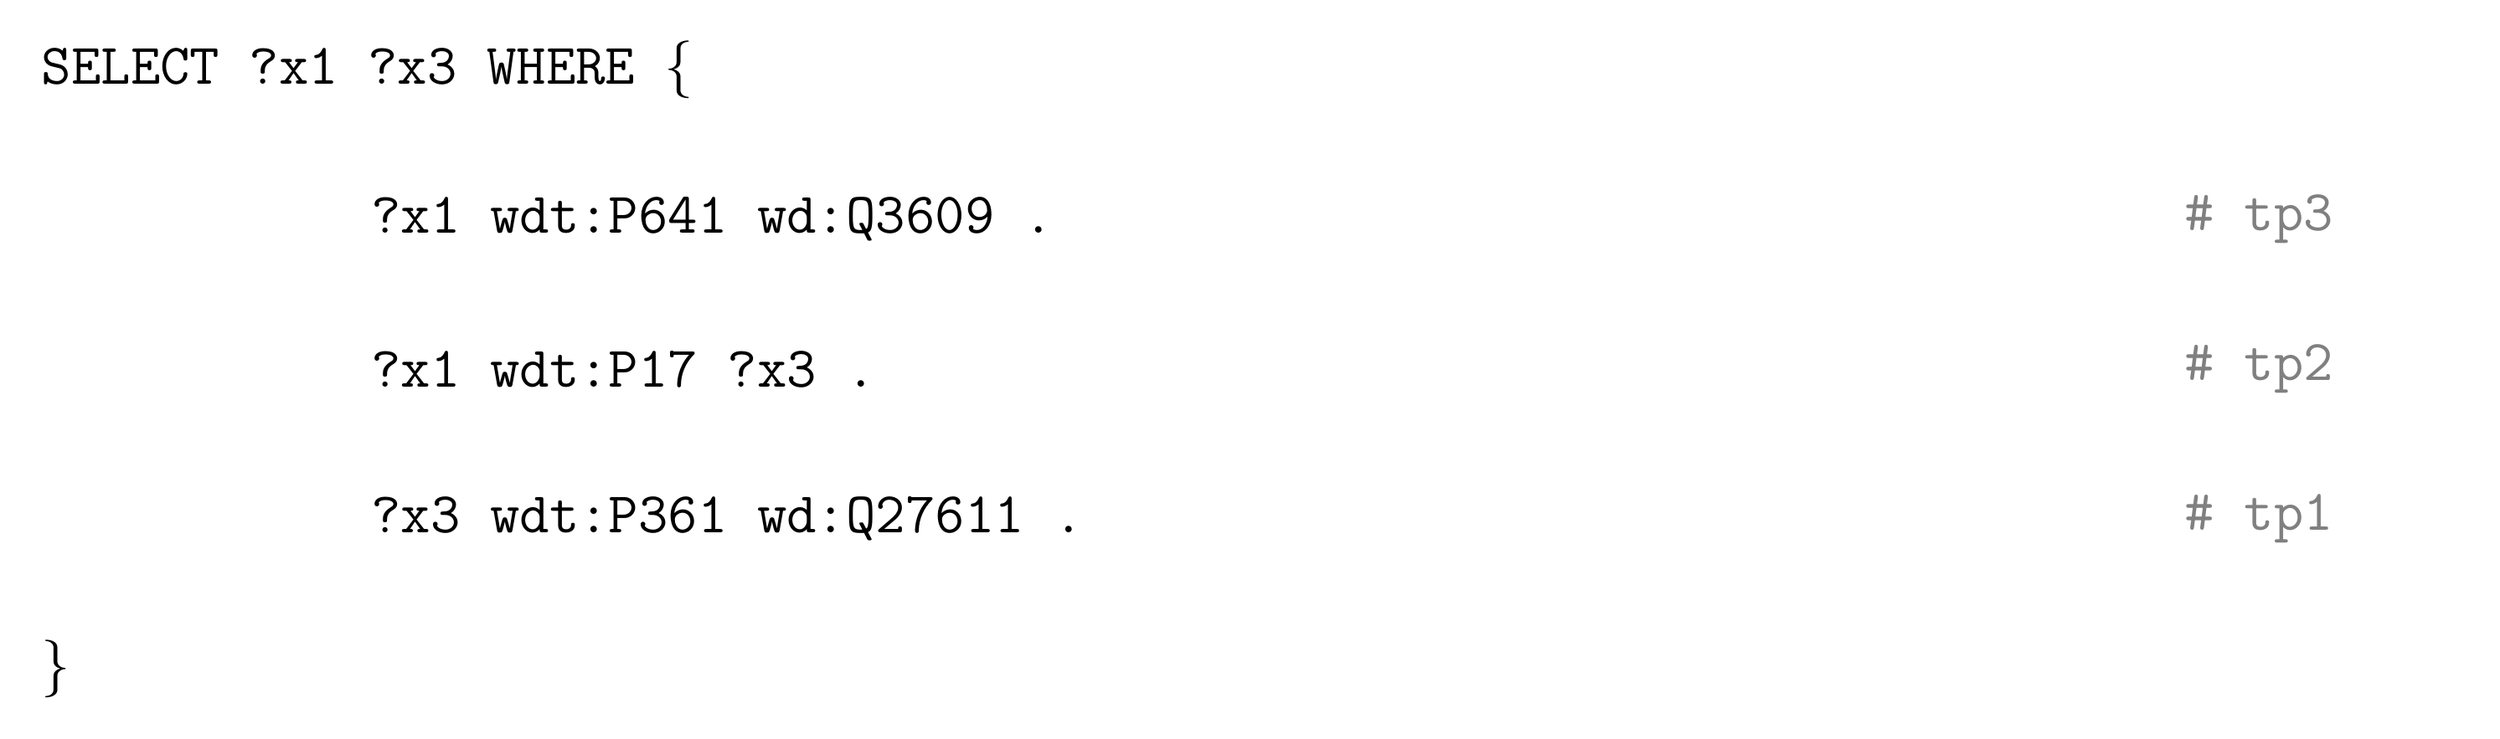
\begin{tikzpicture}
      \newcommand\X{5cm}
      \newcommand\Y{-2.273cm}
      \draw[anchor=west] (0*\X,0*\Y) node {\texttt{\textbf{SELECT} ?x1 ?x3 \textbf{WHERE} \{}};
      \draw[anchor=west] (1*\X,1*\Y) node {\texttt{?x1 wdt:P641 wd:Q3609 .}};
      \draw[anchor=west, color=black!50] (6.5*\X,1*\Y) node {\texttt{\# tp3}};
      \draw[anchor=west] (1*\X,2*\Y) node {\texttt{?x1 wdt:P17  ?x3 .}};
      \draw[anchor=west, color=black!50] (6.5*\X, 2*\Y) node {\texttt{\# tp2}};
      \draw[anchor=west] (1*\X,3*\Y) node {\texttt{?x3 wdt:P361 wd:Q27611 .}};
      \draw[anchor=west, color=black!50] (6.5*\X, 3*\Y) node {\texttt{\# tp1}};
      \draw[anchor=west] (0*\X,4*\Y) node {\texttt{\}}};
      \draw (7*\X,0*\Y) node {\hphantom{positioning}};
    \end{tikzpicture}
  }
  \fbox{
    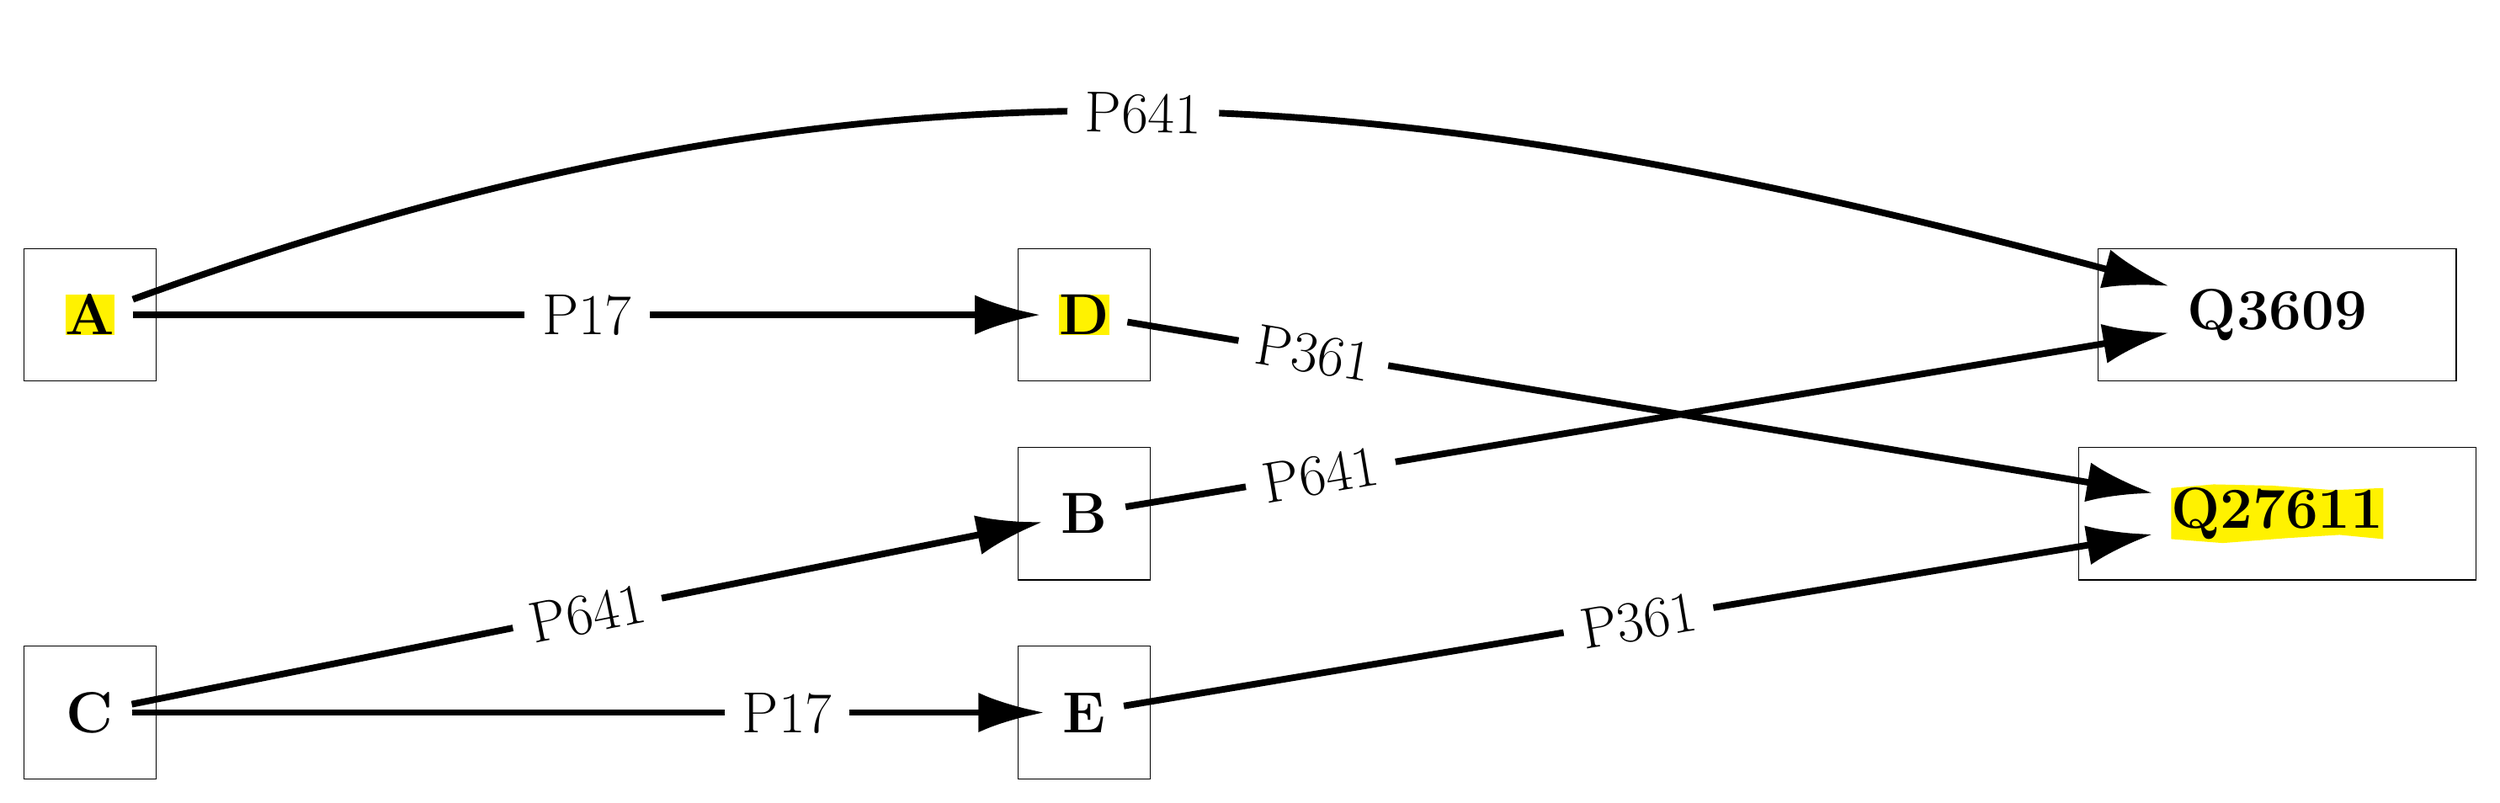
\begin{tikzpicture}
      \thickmuskip=0mu
      \medmuskip=0mu
      \thinmuskip=0mu
      
      \newcommand\X{15cm}
      \newcommand\Y{-3cm}
      \newcommand\PREDICATE{\normalsize}
      \newcommand{\RECTSIZE}{1cm}
      
      \draw (0, 0) node(A){\hlbis{\textbf{A}}} +(-\RECTSIZE, -\RECTSIZE) rectangle +(\RECTSIZE, \RECTSIZE);
      \draw (\X, 0) node(D){\hlbis{\textbf{D}}} +(-\RECTSIZE, -\RECTSIZE) rectangle +(\RECTSIZE, \RECTSIZE);
      \draw (2.2*\X, 0) node(Q3609){\textbf{Q3609}} +(-2.7*\RECTSIZE, -\RECTSIZE) rectangle +(2.7*\RECTSIZE, \RECTSIZE);
      
      \draw (\X, \Y) node(B){\textbf{B}} +(-\RECTSIZE, -\RECTSIZE) rectangle +(\RECTSIZE, \RECTSIZE);
      \draw (2.2*\X, \Y) node(Q27611){\hlbis{\textbf{Q27611}}} +(-3*\RECTSIZE, -\RECTSIZE) rectangle +(3*\RECTSIZE, \RECTSIZE);
      \draw (0, 2*\Y) node(C){\textbf{C}} +(-\RECTSIZE, -\RECTSIZE) rectangle +(\RECTSIZE, \RECTSIZE);
      \draw (1*\X, 2*\Y) node(E){\textbf{E}} +(-\RECTSIZE, -\RECTSIZE) rectangle +(\RECTSIZE, \RECTSIZE);
      

      \draw[->, line width=0.1cm] (A) -- node[fill=white, font=\PREDICATE]{P17} (D);
      \draw[->, line width=0.1cm] (C) -- node[fill=white, sloped, font=\PREDICATE]{P641} (B);
      \draw[->, line width=0.1cm] (C) -- node[fill=white, sloped, font=\PREDICATE, xshift=3cm]{P17} (E);
      \draw[->, line width=0.1cm] (B) -- node[fill=white, sloped, font=\PREDICATE, xshift=-5cm]{P641} (Q3609);
      \draw[->, line width=0.1cm] (E) -- node[fill=white, sloped, font=\PREDICATE]{P361} (Q27611);
      \draw[->, line width=0.1cm] (D) -- node[fill=white, sloped, font=\PREDICATE, xshift=-5cm]{P361} (Q27611);
      \draw[->, line width=0.1cm] (A) to[out=20, in=165] node[fill=white,sloped, font=\PREDICATE]{P641} (Q3609);
      
    \end{tikzpicture}
    }\\
  %
  \adjustbox{max width=0.94\columnwidth}{\textbf{Query $Q_1$: All cycling races of Central America along with
    their respective country. \hspace{6.2em}RDF Graph $G_1$: $A$, $B$,
    and $C$ are cycling sports; $D$ and $E$ are countries of Central
    America.}}
}

\begin{columns}
  \column{0.6}
  \block{}{
    \HRULE
    \begin{center}
      \textit{The estimated cardinality is the inverse probability of sampling}\\
      \hlbis{$P(\gamma_i) = |\left\llbracket tp_1 \right\rrbracket_G|^{-1} \prod_{i=2}^{n}
      |\left\llbracket t_{i-1} \bowtie tp_i \right\rrbracket_G|^{-1}$}.
    \end{center}
    \HRULE
    
    The random walk starts from tp3 with the triple (A, P641, Q3609);
    then instanciating tp2's variable $?x1$ with the node D, it draws
    the triple (D, P361, Q27611); finally instanciating tp1's variable
    $?x3$ with the node D, it assesses that it exists.

    \noindent The cardinality of $Q_1$ is estimated as the inverse
    probability of sampling $\gamma_1$ on graph $G_1$:\\
    \begin{small}
    \begin{tabular}{lll}
      $P(\gamma_1)^{-1} =|\left\llbracket (?x1, \text{P641}, \text{Q3609}) \right\rrbracket_{G_1}| \cdot
       |\left\llbracket (\textbf{A}, \text{P17}, ?x3) \right\rrbracket_{G_1}| \cdot
       |\left\llbracket (\textbf{D}, \text{P361}, \text{Q27611}) \right\rrbracket_{G_1}|
       = 2 \cdot 1 \cdot 1$
    \end{tabular}
    \end{small}
  }
  % \VRULE
  \column{0.4}
  \block{Complexity}{
    We need
    \begin{inparaenum}[(i)]
    \item cardinality estimates at the scale of triple patterns, and
    \item random triples from triple patterns.
    \end{inparaenum}
      
    Common SPARQL query engines -- such as Apache Jena, Virtuoso,
    RDF4J, Blazegraph -- rely on \hlbis{balanced trees}.\\

    We achieve a \hlbis{logarithmic} upper-bound on time complexity !
  }
  \VRULELEFT
\end{columns}

%% \noindent Note that a random walk may fail if it becomes impossible to sample $t_i$ for
%% some $i \leq n$. In this case, its probability $P(\gamma_i)$ of being sampled is 0.
%% For instance, if $t_1 = (B, P641, Q3609)$ is picked in
%% $\llbracket (?x1, P641, Q3609) \rrbracket_{G_1}$
%% instead of $(A, P641, Q3609)$, then the random walk fails because
%% $\llbracket (B, P17, ?x3) \rrbracket_{G_1} = \varnothing$.
%% %
%% To improve the quality of estimates, we compute a set of $k$ random
%% walks $\Gamma = \langle \gamma_1, ..., \gamma_k \rangle$, and the
%% cardinality of $Q$ is estimated as
%% \smash{$|\Gamma|^{-1}\sum_{i=1}^{|\Gamma|} P(\gamma_i)^{-1}$}.
  

%% TODO: add smart client that can perform aggregate
\begin{columns} 
  \column{0.68} 
  \block{Conclusion and Future Work}{
    RAW-JENA provides a \hlbis{\textbf{pay-as-you-go} S-AQP} by implementing \hlbis{random walks on top of
      Apache Jena.} It does not need to reingest the data, everything is
    already there, and it was quite easy to implement.
    The code is open source and available at \dotfill >

    \vspace{0.75em}
    
    However, we need \hlbis{more} than conjunctive queries, and
    \hlbis{more} SPARQL engines with such a feature. We need a \hlbis{standard}!
  }
  \block{}{
    \small
    \vspace{0.55em}
    [1] S. Agarwal, H. Milner, A. Kleiner, A. Talwalkar, M. I. Jordan, S. Madden, B. Mozafari, I. Stoica, \textit{Knowing when you’re wrong: Building fast and reliable approximate query processing systems}.
    
    [2] F. Li, B. Wu, K. Yi, Z. Zhao, \textit{Wander Join and XDB: online aggregation via random walks}.

    [A] Virtuoso, \url{https://docs.openlinksw.com/virtuoso/rndsalltr/}

    [B] Stardog, \url{https://docs.stardog.com/query-stardog/sampling-service\#sampling-service}
  }
  \column{0.34}
  \block{}{
    \begin{center}
    
\includegraphics[width=0.28\textwidth]{images/qr-code.png}
      \small\url{https://github.com/gdd-nantes/raw-jena}
    \end{center}
  }
\end{columns}

\block{References}{
  WanderJoin
  S-AQP
  virtuoso
  stardog
}

\end{document}
